\documentclass[10pt]{beamer}

\usetheme{CambridgeUS}
\usepackage[english, russian]{babel}
\usepackage[utf8]{inputenc}
\usepackage{caption}
\usepackage{minted}
\usepackage{etoolbox}
\usepackage{multicol}
\AtBeginEnvironment{minted}{\singlespacing%
    \fontsize{10}{10}\selectfont}

\title[\href{https://goo.gl/NRgp8K}{https://goo.gl/NRgp8K} (Term 3)]{Суффиксный массив}
\author[Гусев Илья]{Гусев Илья}
\institute[МФТИ] 
{Московский физико-технический институт\\*}
\date{Москва, 2017}
\subject{Computer Science}

\begin{document}

\begin{frame}
  \titlepage
\end{frame}

\begin{frame}{Содержание}
\tableofcontents
\end{frame}

\section{Суффиксный массив}

\subsection{Определение}
\begin{frame}[fragile]{Суффиксный массив - определение}
Дана строка $s$ длины $n$.\\ 
$i$-ый суффикс - $s_i=s[i \ldots n-1]$.\\
Суффиксный массив: $suf=\{i \in [0 \ldots n-1] : \forall j \ne i \quad suf.index[i] < suf.index[j] \rightarrow s_{i} <_{lex} s_{j}\}$\\
То есть, это перестановка индексов суффиксов $s$, которая задаёт порядок суффиксов в порядке лексикографической сортировки.
\end{frame}

\subsection{Пример}
\begin{frame}[fragile]{Суффиксный массив - определение}
Пример:\\
$s = abacaba $\\
$suf = [6, 4, 0, 2, 5, 1, 3]$.\\
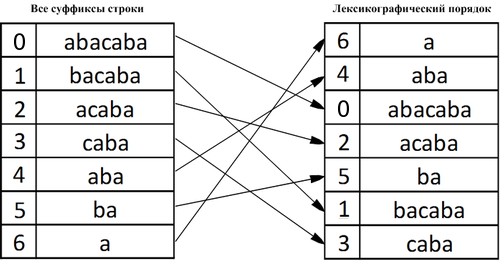
\includegraphics[width=8cm, height=4cm]{Term_3/Source/Pictures/SuffixArray.png}

\end{frame}

\subsection{Алгоритм построения за $O(n \cdot log(n))$}
\begin{frame}[fragile]{Алгоритм построения за $O(n \cdot log(n))$}
Особенности:
\begin{enumerate}
\item Дополняем до циклических сдвигов
\item $c$ - класс эквивалентности по $2^{k-1}$ символам
\item Сортируем первые $2^k$ символов на основе первых отсортированных $2^{k-1}$ и природы суффиксов - O(log(n)) шагов
\item Сортировка пар цифр за $O(n)$
\item Всего $O(n*log(n))$
\end{enumerate}
\end{frame}
\subsection{Алгоритм построения за $O(n*log(n))$}

\begin{frame}[fragile]{Алгоритм построения за $O(n*log(n))$}{Пошаговый пример - 0}
\begin{center}
\begin{tabular}{ c|cccccccc } 
 $p$ & & & & & & & & \\ 
 \hline
 0 & a & b & a & c & a & b & a & \# \\ 
 \hline
 1 & b & a & c & a & b & a & \# & a \\ 
 \hline
 2 & a & c & a & b & a & \# & a & b \\ 
 \hline
 3 & c & a & b & a & \# & a & b & a \\ 
 \hline
 4 & a & b & a & \# & a & b & a & c \\ 
 \hline
 5 & b & a & \# & a & b & a & c & a \\ 
 \hline
 6 & a & \# & a & b & a & c & a & b \\ 
  \hline
 7 & \# & a & b & a & c & a & b & a \\ 
\end{tabular}
\end{center}
\end{frame}

\begin{frame}[fragile]{Алгоритм построения за $O(n \cdot log(n))$}{Пошаговый пример - 1}
\begin{center}
\begin{tabular}{ c|c|cccccccc } 
 $p$ & $c$ & & & & & & & & \\ 
  \hline
 7 & 0 & \# & a & b & a & c & a & b & a \\ 
 \hline
 0 & 1 & a & b & a & c & a & b & a & \# \\ 
 \hline
 2 & 1 & a & c & a & b & a & \# & a & b \\ 
 \hline
 4 & 1 & a & b & a & \# & a & b & a & c \\ 
 \hline
 6 & 1 & a & \# & a & b & a & c & a & b \\ 
 \hline
 1 & 2 & b & a & c & a & b & a & \# & a \\ 
 \hline
 5 & 2 & b & a & \# & a & b & a & c & a \\ 
 \hline
 3 & 3 & c & a & b & a & \# & a & b & a \\ 
\end{tabular}
\end{center}
\end{frame}

\begin{frame}[fragile]{Алгоритм построения за $O(n \cdot log(n))$}{Пошаговый пример - 1}
$k = 0$\\
Для строчки i: \\
$class1_i = c[i]$ \\
$class2_i = c[j: p_j=p_i+2^k=p_i+1]$ \\
\begin{center}
\begin{tabular}{ c|c|cccccccc|c|c } 
 $p$ & $c$ & & & & & & & & & class1 & class2 \\ 
  \hline
 7 & 0 & \textcolor{yellow}{\#} & \textcolor{orange}{a} & b & a & c & a & b & a & 0 & 1 \\ 
 \hline
 0 & 1 & \textcolor{orange}{a} & \textcolor{red}{b} & a & c & a & b & a & \# & 1 & 2 \\ 
 \hline
 2 & 1 & a & \textcolor{blue}{c} & a & b & a & \# & a & b & 1 & 3 \\ 
 \hline
 4 & 1 & \textcolor{magenta}{a} & \textcolor{green}{b} & a & \# & a & b & a & c & 1 & 2 \\ 
 \hline
 6 & 1 & \textcolor{cyan}{a} & \textcolor{yellow}{\#} & a & b & a & c & a & b & 1 & 0 \\ 
 \hline
 1 & 2 & \textcolor{red}{b} & a & c & a & b & a & \# & a & 2 & 1 \\ 
 \hline
 5 & 2 & \textcolor{green}{b} & \textcolor{cyan}{a} & \# & a & b & a & c & a & 2 & 1 \\ 
 \hline
 3 & 3 & \textcolor{blue}{c} & \textcolor{magenta}{a} & b & a & \# & a & b & a & 3 & 1 \\ 
\end{tabular}
\end{center}
\end{frame}

\begin{frame}[fragile]{Алгоритм построения за $O(n \cdot log(n))$}{Пошаговый пример - 2}
Сортируем по паре (class1, class2)\\
\begin{center}
\begin{tabular}{ c|c|cccccccc|c|c } 
 $p$ & $c$ & & & & & & & & & class1 & class2 \\ 
  \hline
 7 & 0 & \# & a & b & a & c & a & b & a & 0 & 1 \\ 
  \hline
 6 & 1 & a & \# & a & b & a & c & a & b & 1 & 0 \\ 
 \hline
 0 & 1 & a & b & a & c & a & b & a & \# & 1 & 2 \\ 
  \hline
 4 & 1 & a & b & a & \# & a & b & a & c & 1 & 2 \\ 
 \hline
 2 & 1 & a & c & a & b & a & \# & a & b & 1 & 3 \\ 
 \hline
 1 & 2 & b & a & c & a & b & a & \# & a & 2 & 1 \\ 
 \hline
 5 & 2 & b & a & \# & a & b & a & c & a & 2 & 1 \\ 
 \hline
 3 & 3 & c & a & b & a & \# & a & b & a & 3 & 1 \\ 
\end{tabular}
\end{center}
\end{frame}

\begin{frame}[fragile]{Алгоритм построения за $O(n \cdot log(n))$}{Пошаговый пример - 2}
$k = 1$\\
Для строчки i: \\
$class1_i = c[i]$ \\
$class2_i = c[j: p_j=p_i+2^k=p_i+2]$ \\
\begin{center}
\begin{tabular}{ c|c|cccccccc|c|c } 
 $p$ & $c$ & & & & & & & & & class1 & class2 \\ 
  \hline
 7 & 0 & \# & a & \textcolor{orange}{b} & \textcolor{orange}{a} & c & a & b & a & 0 & 4 \\ 
  \hline
 6 & 1 & \textcolor{blue}{a} & \textcolor{blue}{\#} & \textcolor{red}{a} & \textcolor{red}{b} & a & c & a & b & 1 & 2 \\ 
 \hline
 0 & 2 & \textcolor{red}{a} & \textcolor{red}{b} & \textcolor{green}{a} & \textcolor{green}{c} & a & b & a & \# & 2 & 3 \\ 
  \hline
 4 & 2 & \textcolor{magenta}{a} & \textcolor{magenta}{b} & \textcolor{blue}{a} & \textcolor{blue}{\#} & a & b & a & c & 2 & 1 \\ 
 \hline
 2 & 3 & \textcolor{green}{a} & \textcolor{green}{c} & \textcolor{magenta}{a} & \textcolor{magenta}{b} & a & \# & a & b & 3 & 2 \\ 
 \hline
 1 & 4 & \textcolor{orange}{b} & \textcolor{orange}{a} & \textcolor{cyan}{c} & \textcolor{cyan}{a} & b & a & \# & a & 4 & 5 \\ 
 \hline
 5 & 4 & \textcolor{yellow}{b} & \textcolor{yellow}{a} & \# & a & b & a & c & a & 4 & 0 \\ 
 \hline
 3 & 5 & \textcolor{cyan}{c} & \textcolor{cyan}{a} & \textcolor{yellow}{b} & \textcolor{yellow}{a} & \# & a & b & a & 5 & 4 \\ 
\end{tabular}
\end{center}
\end{frame}

\begin{frame}[fragile]{Алгоритм построения за $O(n \cdot log(n))$}{Пошаговый пример - 3}
$k = 2$\\
Для строчки i: \\
$class1_i = c[i]$ \\
$class2_i = c[j: p_j=p_i+2^k=p_i+4]$ \\
\begin{center}
\begin{tabular}{ c|c|cccccccc|c|c } 
 $p$ & $c$ & & & & & & & & & class1 & class2 \\ 
  \hline
 7 & 0 & \# & a & b & a & \textcolor{orange}{c} & \textcolor{orange}{a} & \textcolor{orange}{b} & \textcolor{orange}{a} & 0 & 5 \\ 
  \hline
 6 & 1 & \textcolor{red}{a} & \textcolor{red}{\#} & \textcolor{red}{a} & \textcolor{red}{b} & \textcolor{green}{a} & \textcolor{green}{c} & \textcolor{green}{a} & \textcolor{green}{b} & 1 & 3 \\ 
  \hline
 4 & 2 & \textcolor{blue}{a} & \textcolor{blue}{b} & \textcolor{blue}{a} & \textcolor{blue}{\#} & \textcolor{magenta}{a} & \textcolor{magenta}{b} & \textcolor{magenta}{a} & \textcolor{magenta}{c} & 2 & 3 \\ 
 \hline
 0 & 3 & \textcolor{magenta}{a} & \textcolor{magenta}{b} & \textcolor{magenta}{a} & \textcolor{magenta}{c} & \textcolor{blue}{a} & \textcolor{blue}{b} & \textcolor{blue}{a} & \textcolor{blue}{\#} & 3 & 2 \\ 
 \hline
 2 & 4 & \textcolor{green}{a} & \textcolor{green}{c} & \textcolor{green}{a} & \textcolor{green}{b} & \textcolor{red}{a} & \textcolor{red}{\#} & \textcolor{red}{a} & \textcolor{red}{b} & 4 & 1 \\ 
  \hline
 5 & 5 & \textcolor{cyan}{b} & \textcolor{cyan}{a} & \textcolor{cyan}{\#} & \textcolor{cyan}{a} & \textcolor{yellow}{b} & \textcolor{yellow}{a} & \textcolor{yellow}{c} & \textcolor{yellow}{a} & 5 & 6 \\ 
 \hline
 1 & 6 & \textcolor{yellow}{b} & \textcolor{yellow}{a} & \textcolor{yellow}{c} & \textcolor{yellow}{a} & \textcolor{cyan}{b} & \textcolor{cyan}{a} & \textcolor{cyan}{\#} & \textcolor{cyan}{a} & 6 & 5 \\ 
 \hline
 3 & 7 & \textcolor{orange}{c} & \textcolor{orange}{a} & \textcolor{orange}{b} & \textcolor{orange}{a} & \# & a & b & a & 7 & 0 \\ 
\end{tabular}
\end{center}
\end{frame}

\begin{frame}[fragile]{Алгоритм построения за $O(n \cdot log(n))$}{Пошаговый пример - 3}
Сортируем по паре (class1, class2)\\
\begin{center}
\begin{tabular}{ c|c|cccccccc|c|c } 
 $p$ & $c$ & & & & & & & & & class1 & class2 \\ 
  \hline
 7 & 0 & \# & a & b & a & c & a & b & a & 0 & 5 \\ 
  \hline
 6 & 1 & a & \# & a & b & a & c & a & b & 1 & 3 \\ 
  \hline
 4 & 2 & a & b & a & \# & a & b & a & c & 2 & 3 \\ 
 \hline
 0 & 3 & a & b & a & c & a & b & a & \# & 3 & 2 \\ 
 \hline
 2 & 4 & a & c & a & b & a & \# & a & b & 4 & 1 \\ 
  \hline
 5 & 5 & b & a & \# & a & b & a & c & a & 5 & 6 \\ 
 \hline
 1 & 6 & b & a & c & a & b & a & \# & a & 6 & 5 \\ 
 \hline
 3 & 7 & c & a & b & a & \# & a & b & a & 7 & 0 \\ 
\end{tabular}
\end{center}
\end{frame}


\appendix
\section<presentation>*{\appendixname}
\subsection<presentation>*{Useful links}

\begin{frame}[allowframebreaks]
  \frametitle<presentation>{Полезные ссылки}
    
  \begin{thebibliography}{10}
{
  \beamertemplatebookbibitems
  % Start with overview books.
  
  \bibitem{emaxx1}
  \texttt{E-maxx: суффиксный массив}
  \newblock \href{http://e-maxx.ru/algo/suffix_array}{\texttt{http://e-maxx.ru/algo/suffix\_array}}
  
  \bibitem{wiki}
  \texttt{Викиконспекты: суффиксный массив}
  \newblock \href{https://neerc.ifmo.ru/wiki/index.php?title=\%D0\%A1\%D1\%83\%D1\%84\%D1\%84\%D0\%B8\%D0\%BA\%D1\%81\%D0\%BD\%D1\%8B\%D0\%B9_\%D0\%BC\%D0\%B0\%D1\%81\%D1\%81\%D0\%B8\%D0\%B2}{\texttt{https://neerc.ifmo.ru/wiki/index.php?title=Суффиксный\_массив}}
}
    
  \end{thebibliography}
\end{frame}

\end{document}


